\documentclass{article}\usepackage{graphicx}
\usepackage[a4paper, margin=1in]{geometry}
\usepackage{hyperref}
\usepackage{titlesec}
\usepackage{todonotes}

\titleformat{\section}{\large\bfseries}{}{0em}{}

\title{\textbf{Chat Vibe Check: Process Book}}
\begin{document}
\maketitle

\section{Project Metadata}
\begin{itemize}
    \item \textbf{Project Title:} Chat Vibe Check
    \item \textbf{Team Members:} 
    \begin{itemize}
        \item Deepa Rukmini Mahalingappa (34040788, drukminimaha@umass.edu)
        \item Benjamin Ibasco (28561432, bibasco@umass.edu)
        \item Javin Mendiratta (33328658, jmendiratta@umass.edu)
    \end{itemize}
   
    \item \textbf{Project Repository:} \href{https://github.com/bibascoumass/chat-vibe-check}{Link}
\end{itemize}

\section{Overview and Motivation}
In the current technical climate, everyone is messaging everyone. The messages we send and receive can have everlasting impacts on our social, personal, and even professional life. We believe it is very important to understand the intricacies of text conversations with others. As we explore the various metrics of these messages, it becomes important to interpret associated behavioral patterns, insights, and attachment styles to facilitate personal and interpersonal growth and communication. Most modern chat visualization tools primarily provide visualizations on simple metrics such as popular word counts, and message counts over time. In reality, however, there are many intricacies when it comes to trying to break down what may seem like a simple conversation. Response times, sentiment, and the overall flow of conversation can help with understanding hidden nuances in interpersonal relationships, and even hidden facets of our own personalities. As such, we aim to create a tool that can begin bridging that gap- to approach these messages from a more psychological perspective- analyzing not just what you're saying, but what you mean. We are complex beings, and we hope this creation of ours can help, even just a little bit, in better understanding ourselves.

\section{Related Work}
We were inspired by looking at our own lives. We all have many different messaging apps with various people and personalities. Even our group chat for this project falls under this purview! Additionally, while looking into articles such as \href{https://www.businessinsider.com/chatgpt-analyze-chat-history-between-girlfriend-boyfriend-2025-3}{I asked Chat-GPT to analyze my texts}, and \href{https://www.youtube.com/watch?v=PROIhoYPaXM}{What does your chat history reveal about you?}, we saw that this conundrum was something on the minds of many people. With the advent of social media, we wanted to be able to contribute towards answering this complex, intricate ask with our own understandings from class lectures on using visualizations to communicate information and understandings to others.


\section{Questions}
Our project initially focused on answering the following questions:
\begin{itemize}
  \item \textbf{What about conversations can we analyze} that may indicate what a person's attachment style is? 
  \item \textbf{How do sentiments change based on time}? 
  \item \textbf{How have response times changed over time?} 
  \item What is each user's estimated attachment style? 
\end{itemize}
After working on the project, we were able to answer and expand upon the first three questions:
\begin{itemize}
  \item \textbf{What about conversations can we analyze?}- We focused on analyzing the sentiment and response times. As we worked on this question, we also game across the question of \textbf{How large of conversations can we analyze, and how many people can be in these conversations?}
  \item \textbf{How do sentiments change based on time?} We realized that another key aspect to consider is the topic of conversations, adding the question of \textbf{How do sentiments change based on the topic of conversation?} 
  \item \textbf{How have response times changed over time?} Similar to the previous, we also begun to ask \textbf{How do response-times} (or more specifically, sparsity of active conversation) \textbf{change based on the topic of conversation?} 
  \item What is each user's estimated attachment style? 
\end{itemize}
Unfortunately, we did not truly get to solidly answering the fourth question. We learned that \textbf{Analyzing an attachment style is extremely complex}- we did not have the time nor capabilities to do so with realistic accuracy in our provided time-frame. While shallow analysis is possible by viewing our presented graphics, we could not devise an algorithm that could take in the data or analyzed metrics and yield and "attachment style".


\section{Data}
We were unfortunately not able to get any users to volunteer to share their own data which was understandable. In retrospect, we realize basing the project primarily on static data should've been the focus since a working prototype of the visualizations would've been the bare minimum requirement needed to get users interested or comfortable to share their data and so really the upload and doing insights dynamically should've been a goal in the next phase of this project if it were to continue.
\newline

So we pivoted to relying on static data and settled on a dataset of over one million two-person chat logs related to Ubuntu technical support (\href{https://www.kaggle.com/datasets/rtatman/ubuntu-dialogue-corpus/data}{Kaggle URL for Ubuntu Dialogue Corpus}). We chose this dataset because the conversations were one-on-one only, the longest conversations had a lot of data (over ~1K messages), and it was really the only chat based dataset we could find in English as all other chat based datasets we found were in different languages. 

\section{Data Processing}
The chat conversation data is over 2.7Gb and composed of over 26 million messages split across 3 CSV files. We then extracted the 50 longest conversations into their own CSV files using a Python script which amounted to over 38 thousand messages and 4.1Mb to avoid our application having to do this filtering work. Since the focus is the individual conversation level insights we could gain, we focused on visualizing the conversations that could give us the most data individually rather than trying to visualize all of the conversations in the dataset. 
\newline

We primarily used three derived attributes for our visualizations, sentiment score, response time. and topic. Sentiment score for a message was the average sentiment score for all the words in the message which was measured using the Sentiment Node.js module which uses AFINN-165 wordlist and the Emoji Sentiment Ranking to perform sentiment analysis. Response time for each message was simply getting the time elapsed since the last message from the other user. As for topic, we experimented with trying to derive the topic from the content of the conversations and trying detect the type of technical support issue each one was but had to settle for manually setting the topics as we needed to prioritize the core visualizations that didn't require topics to provide insights. There were optimization challenges with measuring sentiment and response time as well for example, we could've improved the sentiment measurement by incorporating the context of the use of each word into the sentiment rather than each of them individually.
\newline

 In retrospect, although this project was a good learning lesson on the challenges of working on derived attributes, we realized that we should've ensured that our visualization did not entirely rely on derived data as wrestling with optimizing the measurement alone of it can be tricky in order to get the most meaningful insights.

\section{Visualization Design}

\section*{Design Evolution}
The project aimed to extract and visualize emotional patterns from chat data in a way that is easy to interpret, interactive, and actionable. Our design evolved significantly from the initial proposal as we explored more effective ways to represent time-based and user-based sentiment trends.


\begin{itemize}
    \item \textbf{Initial Visualizations Considered:}
    \begin{itemize}
        \item Bar charts to show average sentiment per user or per day.
        \item Line charts for sentiment flow over time.
        \item Pie charts to show distribution of sentiment types.
        \item Snakey Diagram showing the flow of conversation state transitions from neutral to conflict to resolution.
    \end{itemize}

    \item \textbf{Final Visualizations Used:}
    \begin{itemize}
        \item \textbf{Heatmap:} Showcased sentiment variation across time periods (e.g., hourly/daily), helping identify emotional peaks.
        \item \textbf{Scatter Plot - Response Time vs Sentiment:} Revealed correlation between emotional intensity and reply latency.
        \item \textbf{Scatter Plot - Timestamp vs Sentiment:} Illustrated sentiment flow throughout the conversation, supporting detection of escalating or resolving emotional trends.
        \item \textbf{Chat Parser Table:} Provided a clean, searchable layout of individual messages with timestamps, user labels, and sentiment tags.
    \end{itemize}    

    \item \textbf{Deviations from Original Proposal:}
    \begin{itemize}
        \item Initially proposed line charts were replaced by scatter plots, which better captured the irregular and message-level nature of chat data.
        \item We're currently playing around relating time, topic and sentiment instead all in one chart rather than having a two separate ones for topic and then for time.
        \item The most basic implementation for showing the chat is currently just having it as a separate page but we will look into the displaying it as the user clicks on messages. 
    \end{itemize}
\end{itemize}
 \section*{Visualizations Used}

\begin{itemize}
    \item \textbf{Heatmap: Sentiment vs Time}
    \begin{itemize}
        \item \textbf{Design Goal:} To identify how sentiment changes over time (across hours or days), highlighting peak emotional periods like high negativity during specific hours.
        \item \textbf{Color Mapping:}
        \begin{itemize}
            \item \textcolor{red}{Red} = Negative
            \item \textcolor{green}{Green} = Positive
            \item \textcolor{gray}{Gray} = Neutral
        \end{itemize}
    \end{itemize}
    
    \item \textbf{Scatter Plot: Response Time vs Sentiment}
    \begin{itemize}
        \item \textbf{Design Goal:} To explore whether the speed of replies correlates with emotional tone, revealing patterns like faster responses during emotional conversations.
        \item \textbf{Design Enhancements:}
        \begin{itemize}
            \item Color-coded sentiment points for clarity.
            \item Tooltips on hover for detailed insights.
            \item Filter options by user or time range.
        \end{itemize}
        \item \textbf{Design Principles Used:}
        \begin{itemize}
            \item Data-ink ratio for clean visualization.
            \item Pre-attentive processing with color and shape to distinguish sentiment.
        \end{itemize}
    \end{itemize}
    
    \item \textbf{Scatter Plot: Timestamp vs Sentiment}
    \begin{itemize}
        \item \textbf{Design Goal:} To display sentiment flow chronologically over the chat session, allowing trend detection like escalating negativity or emotional recovery.
        \item \textbf{Design Decisions:}
        \begin{itemize}
            \item Smooth timeline across X-axis.
            \item Hover details with sentiment classification.
        \end{itemize}
        \item \textbf{Design Principle Used:}
        \begin{itemize}
            \item Temporal alignment of visual elements for easy scanning.
            \item Consistent color scale to maintain cognitive ease.
        \end{itemize}
    \end{itemize}
    
    \item \textbf{Chat Parser with Sentiment Tags}
    \begin{itemize}
        \item \textbf{Design Goal:} To convert raw chat into a clean, readable, and searchable table with labeled sentiment.
        \item \textbf{Features:}
        \begin{itemize}
            \item Each message row includes: Timestamp, User, Message, and Sentiment Score (with tag).
            \item Sentiment tags are color-coded.
            \item Optional search/filter by user or sentiment type.
        \end{itemize}
        \item \textbf{Design Principles Used:}
        \begin{itemize}
            \item Clarity and hierarchy through formatting, spacing, and alignment.
            \item Redundancy principle — sentiment shown via both text and color for accessibility.
        \end{itemize}

        
    \end{itemize}
\end{itemize}



\section*{Implementation}
Our implementation, at the current stage, features a home page for uploading documents, and 4 main features across 3 sub-pages. We plan to add more implementations, interactivity, and design consistency before out final submission.
\\\\
Before any of the views can be made, the user must upload their chat log to the website in order for it to be analyzed and parsed on the backend. As of now, our inputs must be a csv with the following format: (!). However, we plan to extend the input types to a more generic implementation.
\begin{itemize}
    \item Home page: This is the page where the user will select the file and upload it. After uploading the file, they can then choose a view from the toolbar. We will decide on and create a default view to show the user immediately upon upload to ensure a smoother and more natural experience. 
    \item 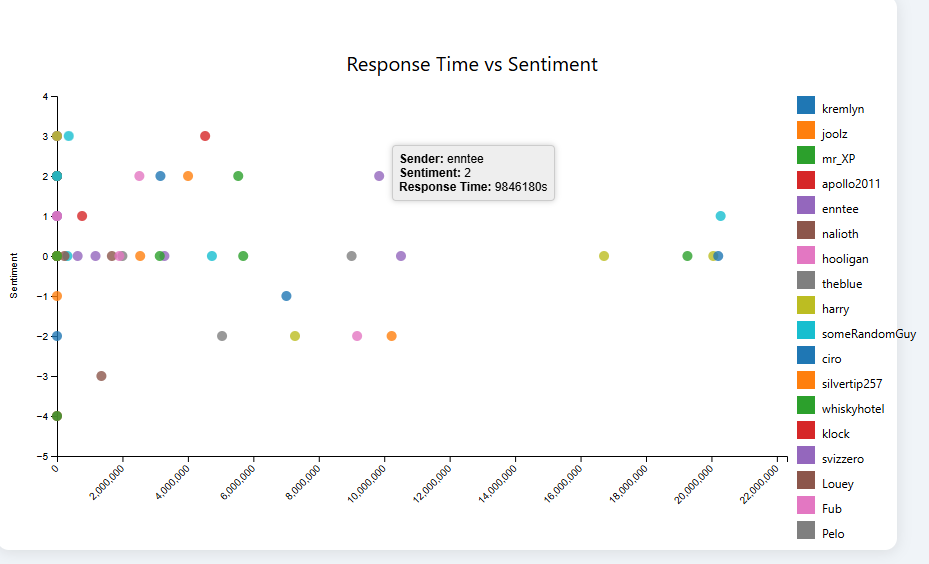
\includegraphics[width=10cm]{./Latex Images/Responsetime timeline ss.png}
    \item Time (X-axis) vs Sentiment (Y-axis) Scatterplot: Each point represents a message and each point is labeled by user. This plot is meant to showcase the various sentiments shown in the conversation over time, with colors of nodes corresponding to the users and the y-axis showing sentiment (positive vs negative). Each node (message) also displays the sender, sentiment, and timestamp when hovered over. Currently, the graph looks a little cluttered and is working for group messages. We want to see how it will look for smaller chats eventually and add a feature to specify members for group chats.
    \item 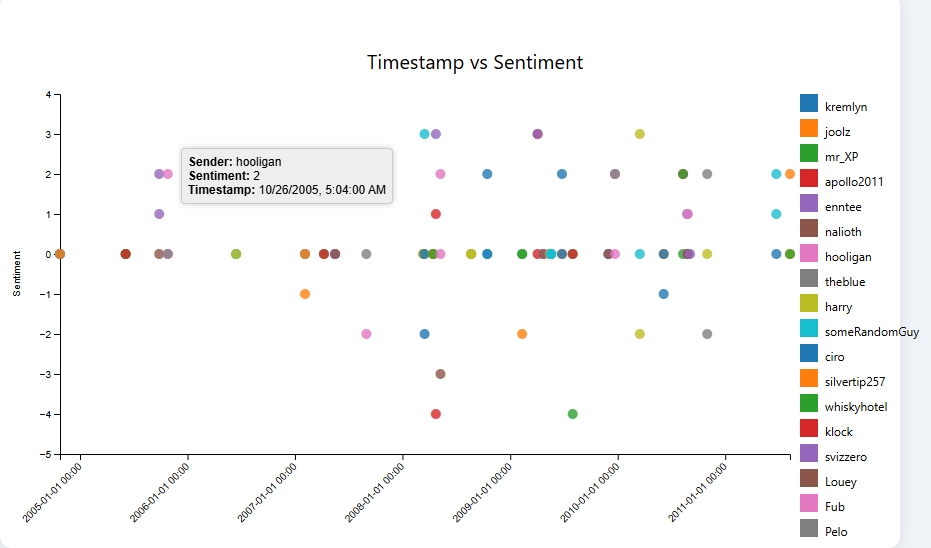
\includegraphics[width=10cm]{./Latex Images/Timeline Sentiment ss.png}
    \item Response Time (X-axis) vs Sentiment (Y-axis) Scatter Plot: Each point represents a message and each point is labeled by user. This plot is meant to showcase the various response times shown in the conversation for varying sentiments, with colors of nodes corresponding to the users and the y-axis showing sentiment (positive vs negative). Each node (message) also displays the sender, sentiment, and response time when hovered over. Currently, the graph is a little confusing to properly interpret. We are considering switching the axis to make response time the dependent variable, so we can analyze if different sentiments influence response time. We may expand this to include topic instead of sentiment as an axis, and explore different chart styles.
    \item 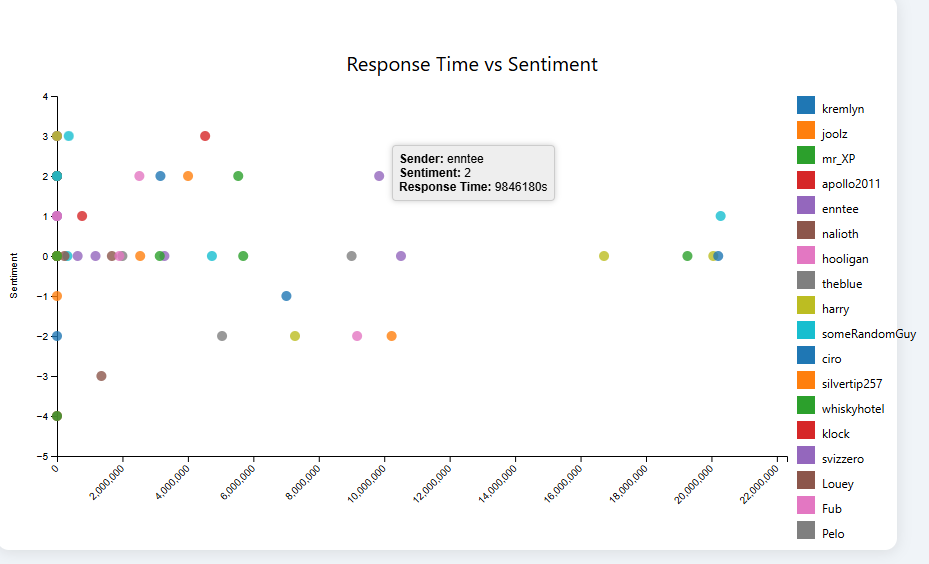
\includegraphics[width=10cm]{./Latex Images/Responsetime timeline ss.png}
    \item NEEDS WORK: Topic (X-axis) vs Sentiment (Y-axis) Heatmap: This graph is incorrect at the moment, as we need to update it. Currently we have the x-axis showing the timestamp of the message and the y-axis being discrete with certain topics. As such, a different chart style, where topics are more distinctly serrated may be in order. Additionally, our code that determines topics is somewhat faulty, and we need to broaden our range of topics to identity- right now every conversation is being placed in the "other" category. 
    \item 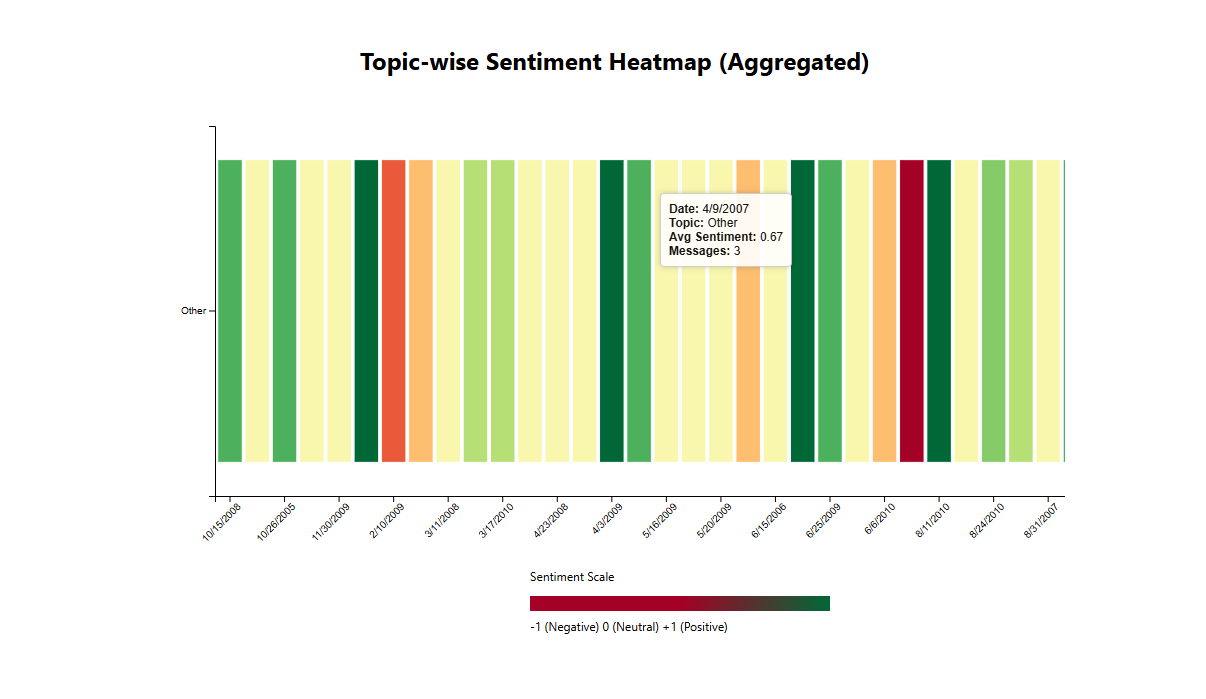
\includegraphics[width=10cm]{./Latex Images/Sentiment heatmap ss.png}
    \item Conversation Display: This visual simply lists out the entire chat conversation in a scroll-able text box, showing the message and it's corresponding sentiment. This is to provide a familiar interface to the user, while providing a more "overall" view of the data. We will need to incorporate pages or some effective way to split up the conversation for larger datasets.
    \item 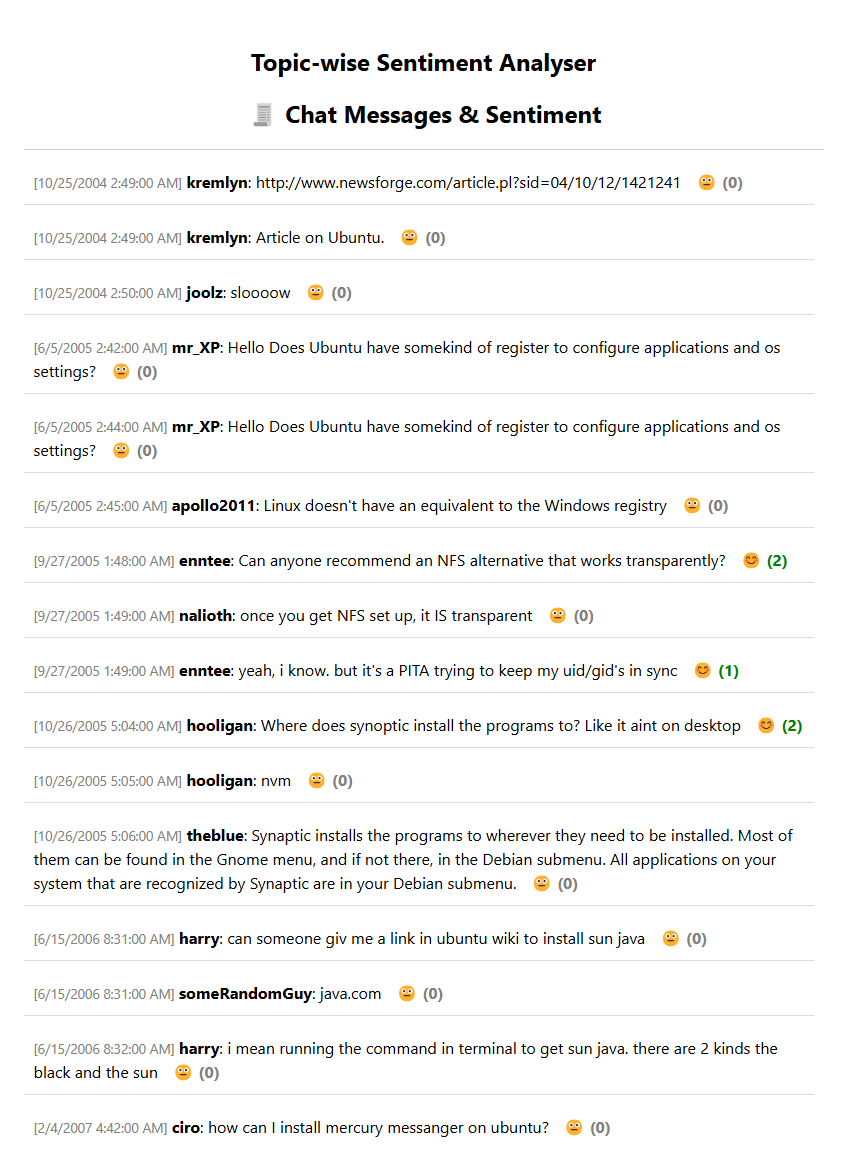
\includegraphics[width=10cm]{./Latex Images/Chat log ss.png}
\end{itemize}


\section{Evaluation}
We learned many things, and learned that we do not know many things, in the process of constructing our visualizations. When it comes to our research questions, we answered them using three visualizations:
\begin{itemize}
    \item Sentiment Heatmap: 
    \begin{itemize}
        \item We designed a sentiment heatmap that displays the sentiments associated with topic. This aimed to answer our \textbf{How do sentiments change based on topic of conversation?} and \textbf{How do response-times change over time based on the topic of conversation?} questions. We learned that many topics, when looking at their average sentiment, were actually more negative or neutral in nature. We believe that this may have been in part due to the way in which we split our topics, and also due to the data itself. We noticed that topics such as food and emoticons had a much higher average sentiment, as those are things usually associated with relaxation and positive experiences. On the other hand, topics such as Education and Tech Support has much more negative sentiment, likely due to the fact that messages on those topics typically deal with frustrations and troubles. Finally, we noticed that topics that fell under Requests were the most positive- politeness when asking for help is part of common decency, and this seems to reflect in our data- our group chatters were quite polite.
        \item Our visualization does have some limitations and imperfections. Our heatmap has a limited number of hard-coded topics that we try to assign to the messages. We attempted to use ML to do topic-matching and text analysis, but were unable to get desirable results. Our time scatterplot is but finicky with display and get extremely crowded if a high-volume element is displayed.   
    \end{itemize}
    \item Scatterplot of Sentiment over Time:
    \begin{itemize}
        \item We created two scatterplot that display the sentiments and response-times of messages over time. The data displayed can be filtered based on topic and conversation. This aimed to answer our \textbf{How do sentiments change based on time?} and \textbf{How do response-times change over time?} questions. Our data provided a lot of insight on how certain topics had more or less responses, and how some of the conversations (when filtered), showed a different spread of sentiment and response-time, leading to us finding different correlations between the two dependent metrics. For example, longer response-times usually meant that there was a lower neutral sentiment associated with the message, as either the responder was upset or disinterested in the conversation, leading to the larger lag in response. 
        \item Our scatterplot limitations primarily fall under the limits of our data itself. As previously mentioned, we did not implement the most effect topic-analysis into our code, and our data could have been larger in size to provide for variety and thus more insight. However, we believe our scatter-plots are a great proof-of-concept towards our ultimate vision regarding this project.
    \end{itemize}
    \item Conversation Log:
    \begin{itemize}
        \item This was a much simpler visualization that simply displays the chat logs used for the visualization as a scroll-able text format, along with the ability to see the "longest conversation", something we were interested in when approaching the \textbf{How large of conversations can we analyze, and how many people can be in these conversations?} question. 
        \item The main limitation with this visualization is the inability to filter or search through the display logs, making it difficult to actually gain any insight just by looking at it (besides the longest conversation). This is something we wanted to implement, but did not prioritize as it was not the main focus of our website.
    \end{itemize}
\end{itemize}


\end{document}
